\documentclass[tikz]{standalone}
\begin{document}
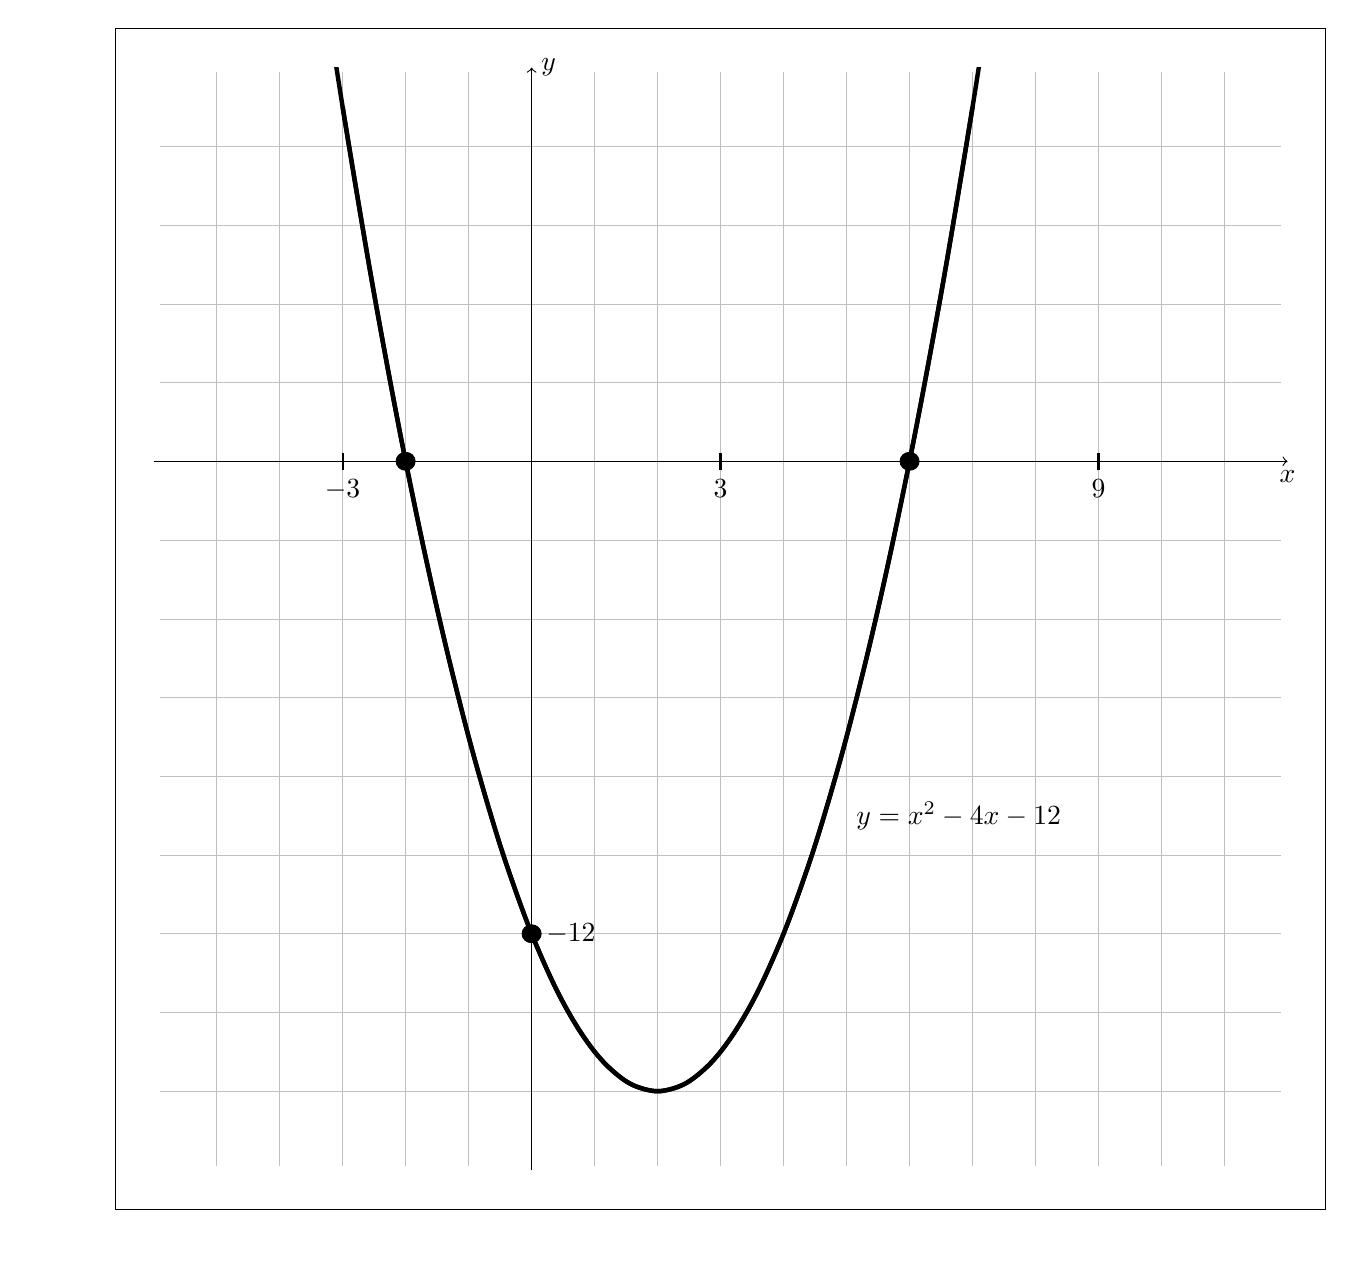
\begin{tikzpicture}[xscale=0.8,yscale=0.5]

\draw[black,fill=white] (-6.6,-19) rectangle (12.6,11);
\draw[very thin,color=lightgray,xstep=1,ystep=2] (-5.9,-17.9) grid (11.9,9.9);

\draw[->] (-6,0) -- (12,0) node[below] {$x$};
\draw[->] (0,-18) -- (0,10) node[right] {$y$};
\draw[domain=-3:7,smooth,variable=\x,black,ultra thick] plot ({\x},{\x*\x - 4*\x - 12});
       
\node[right] at (5, -9){$y = x^2-4x-12$};

%\draw [fill=black,thick] (-2,0) circle [radius=0.15];
%\draw [fill=black,thick] (6,0) circle [radius=0.15];
%\draw [fill=black,thick] (0,-12) circle [radius=0.15];
\draw [fill=black] (-2,0) ellipse [x radius = 0.15, y radius = 0.225];
\draw [fill=black] (6,0) ellipse [x radius = 0.15, y radius = 0.225];
\draw [fill=black] (0,-12) ellipse [x radius = 0.15, y radius = 0.225];

% tick marks
\foreach \x in {-3,3,9} 
	\draw [thick] (\x cm,6pt) -- (\x cm,-6pt) node[below] {$\x$};
\foreach \y in {-12} 
	\draw [thick] (-2pt,\y cm) -- (2pt,\y cm) node[right] {$\y$};
	
\clip (-8,-20) rectangle (12,10);
\draw[domain=-4:8,smooth,variable=\x,black,ultra thick] plot ({\x},{\x*\x - 4*\x - 12});

\end{tikzpicture}
\end{document}
